\subsubsection{Channel Characterization, Electromagnetics, Prototype System Development}
\index{Wallace, Jon}

\paragraph{Research Team}
Wallace, Jon (Professor)\\

Research combines the diverse areas of electromagnetics and
propagation, signal processing, and communications, to allow more
accurate modeling of realistic communications systems, revealing how
to optimize the performance of complex systems as a whole rather
than just the constituent parts.  This research involves a strong
experimental component, allowing results to be based on real-world
experiments and measurements and not just theoretical analysis. This
effort has led to the development of a number of prototype
multiple-input multiple-output (MIMO) wireless channel sounders and
the fabrication of RF/microwave antennas and components,
facilitating the development of accurate channel models and
revealing the impact of factors such as antenna mutual coupling,
directivity, and polarity. The work also encompasses the development
of real-time systems based on DSP and FPGA architectures for
implementing proposed communications algorithms as well as advanced
measurements techniques.

\paragraph{Highlights}

The work during 2006 has focused primarily on understanding the
complex behavior of time-varying MIMO wireless channels.  The rate
of time variation determines whether the MIMO communications channel
can be adequately tracked, allowing high throughput to be achieved
with the multiple antennas.

\begin{figure}[ht]
  \begin{center}
    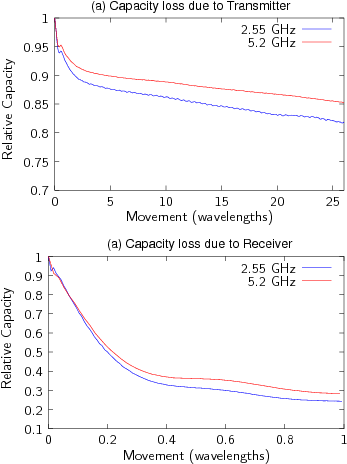
\includegraphics[width=6cm]{wallace_cap_deg.png}
    \caption{Capacity loss from time-varying channel with receiver
    movement due to channel errors at (a) transmitter and (b) receiver}
   \label{fig:wallace_cap_deg}
   \end{center}
\end{figure}

Measurement and analysis of time-varying channels in indoor and
outdoor environments at different frequencies revealed that for
moving users, the channel must be sampled at the receiver
approximately every 0.1 wavelength or shorter for high-capacity
communications, as depicted in Fig.~\ref{fig:wallace_cap_deg}.  It
was also found that channel information at the transmitter is less
critical and can be updated at the slower rate of every 1 wavelength
for high capacity.

This study on channel time-variation also led to metrics that quantify
the impact of the temporal variability as well as accurate methods of
capturing this behavior in computer simulations.  For very rapidly
fading channels (where learning the channel is not possible) it was
discovered that mutual coupling of the transmit array is a critical
factor affecting the system performance, and that not including
mutual coupling in the system model leads to erroneous conclusions
about the optimal configuration of the transmit antenna array.

\begin{figure}[ht]
  \begin{center}
    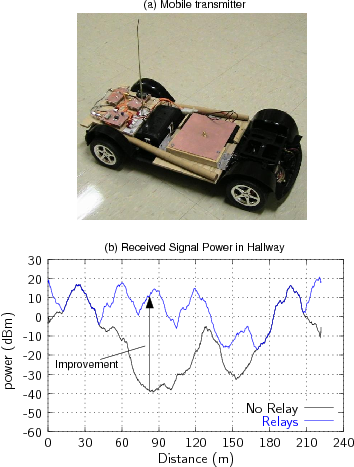
\includegraphics[width=6cm]{wallace_relay2.png}
    \caption{System for rapid shadowing/pathloss measurements and possible
    improvement using relays for a hallway environment}
   \label{fig:wallace_relays}
   \end{center}
\end{figure}

Additional channel modeling work done in collaboration with the
University of Pretoria, South Africa, has demonstrated interesting
properties of indoor propagation channels.  It has been discovered
that the multipath structure, antenna correlation, and channel
capacity are very similar, even when the center frequency is scaled.

Defense-related contract work  was done for San Diego Research
Corporation, USA, whose primary goal was to quantify how the
blockage (or shadowing) of electromagnetic signals in urban
environments limits communications reliability, and whether this
could be improved by robotic relays.  As depicted in
Fig.~\ref{fig:wallace_relays}, a transmitter operating at 300 MHz,
900 MHz, and 2 GHz, was mounted on a remote control car and the
signal strength was measured on a fixed receiver.  The car was
driven in many different scenarios: indoor hallway, indoor room,
outdoor-to-indoor channels, behind automobile, under automobile,
etc. Analysis of the resulting shadowing versus position revealed
that shadowing can cause a drop of 10-30 dB when going around a
corner or behind an automobile.  A simple daisy-chain relay model,
however, indicated that self-configuring robotic relays may be
effective in allowing reliable communications in these environments.


In the future, the main focus is  building up new experimental
capability for ultrawideband multiple antenna channel sounding and
cognitive radio, as well as forming collaborative relationships with
other key researchers in Germany and Europe.

%Pictures are to be included via:
%
%\begin{figure}[ht]
%  \begin{center}
%    \includegraphics[width=6cm]{profxxx-figx.jpg}
%    \mycaption{ xxx )}\label{fig:profxxx}
%   \end{center}
%\end{figure}

% \paragraph{Organization}
% list the (research) events you have organized, if any,
%
%\begin{enumerate}
%\item  xxx
%\item  xxx
%\end{enumerate}

 
\paragraph{Collaborations}
\begin{enumerate}
\item {\sl University of Pretoria, South Africa} \\ B. T. Maharaj and L. P. Linde \\ Indoor Channel Measurement and Modeling
%\item {\sl Institution} \\ Partner \\ Research Topic \ Collaboration
\end{enumerate}

%\paragraph{Grants}
%% list the running grants in 2005, if none have been received, please delete this
%% subsection.
%\begin{enumerate}
%\item {Funded by} ``Proposal ��
%\item {Funded by} ``Proposal ��
%\end{enumerate}

%\paragraph{Awards, Prizes}
%% list the grants you have received in 2005, if none have been received, please delete this
%% subsection.
%\begin{enumerate}
%\item
%\item
%\end{enumerate}

%\paragraph{Publications}
  \nocite{wallace_06bWALa,wallace_069WAL,wallace_06bWALb}

%Publications should be delivered as a separate file (naming
%convention profxxx.bib. See description by R. Helling. Please make
%sure that all your publications are referred to in the TiX file.
%This can either be in form of a \cite{profxxxkey} or as a
%\nocite{profxxxkey} in the end. A publication which is not
%reffered to on the LaTeX file doesn't produce any output in the
%report.
